\chapter{Conclusion}
\label{chap:conclusion}

As a conclusion I am going to briefly summarize the mapping and the motion planning algorithms, and evaluate whether they have achieved the expected results. The main task of the project was to create two ROS nodes that can be integrated into an existing system. The tasks of these two nodes were to separate the static and dynamic objects in the map, and calculate actuations that avoid these obstacles.

\section{Mapping results}
The aim of the mapping node was to find the moving objects in the environment, based on LIDAR scans, and to separate them from the static parts of the map. The algorithm converted the LIDAR measurements into absolute map points, than created a differential grid - basically a map, with the high values not marking objects like a regular map, but marking movements. The algorithm found the possible dynamic point candidates based on this grid. After the candidates have been selected, the algorithm created groups among the measured points, based on the positions. Relying on these groups being valid, and the assumption that points in the same group must be still or moving in the same direction, speed vectors were calculated for the groups. The groups with speed larger than a minimum value (which may be caused by measurement noise) became the moving objects, and the points inside these groups were marked dynamic. Every other measurement was treated non-moving, and therefore placed in the static map. The static map building is as straightforward as it can be - every static measurement creates a free ray in the map, starting from the position of the LIDAR and ending at the measured point.

The results of the mapping and the separation of static and dynamic points are presented by an example with a valid use-case. The scenario is the following. The car is standing in a closed room, the distance from the walls are smaller than the LIDAR's range. There is one other object in the room, in the simulation, this is a ball, its size similar to the car's. The ball is standing in one place at first, but after a while, it start moving in a straight path with constant speed. Finally, the car starts moving as well - first in a straight path, then turning.

\ref{mapping_demo_start} presents the initial situation of the demonstration. The left image shows the simulation - the car is standing in the middle of the room, the object in the top left corner is not moving yet. On the right image, the created static map is visible. The number of unknown (grey) grid points is large at this state of the simulation, it will dramatically decrease once the car starts moving. This effect is caused by the LIDAR's finite angular resolution and ray characteristics. The black grid points represent statically occupied positions. All the walls are marked static, and the ball as well.

\begin{figure}[!ht]
    \centering
    \subfloat[Gazebo simulation]
    {
        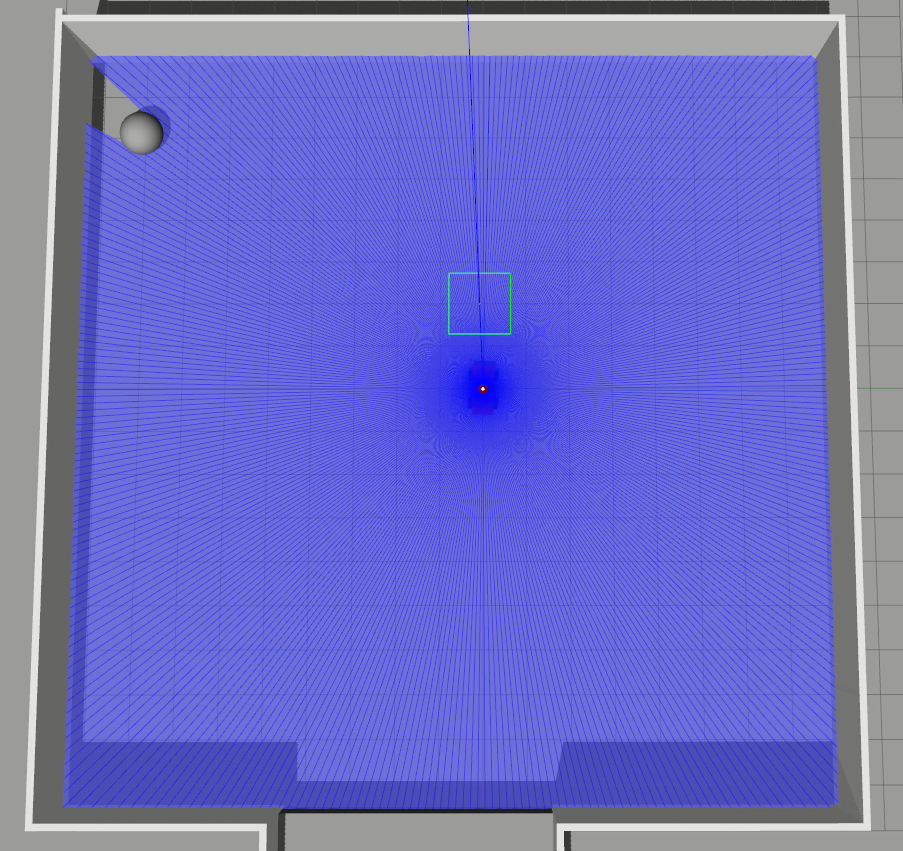
\includegraphics[height=70mm]{figures/raw/mapping_demo/gazebo_start.png}
        \label{mapping_demo_gazebo_start}
    }
    \subfloat[rviz visualization]
    {
    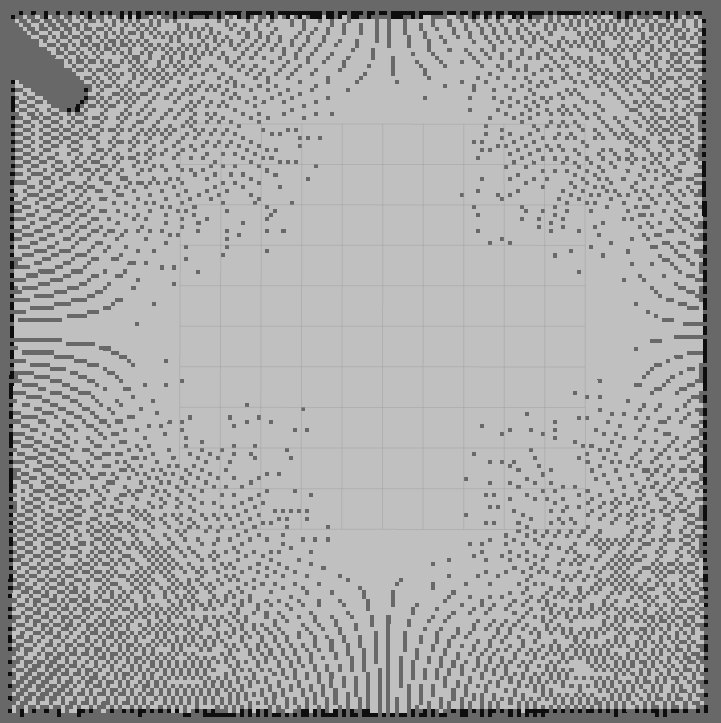
\includegraphics[height=70mm]{figures/raw/mapping_demo/rviz_start.png}
        \label{mapping_demo_rviz_start}
    }
    \caption{Initial state - ball is still}
    \label{mapping_demo_start}
\end{figure}

Once the ball starts moving (\ref{mapping_demo_ball_moving}), it stops being marked as static, but is handled as a moving object. The static block at the top left corner has been removed, and the ball is displayed using the dynamic visualization toolset - a sphere and an arrow, representing the ball's area and speed vector.

\begin{figure}[!ht]
    \centering
    \subfloat[Gazebo simulation]
    {
        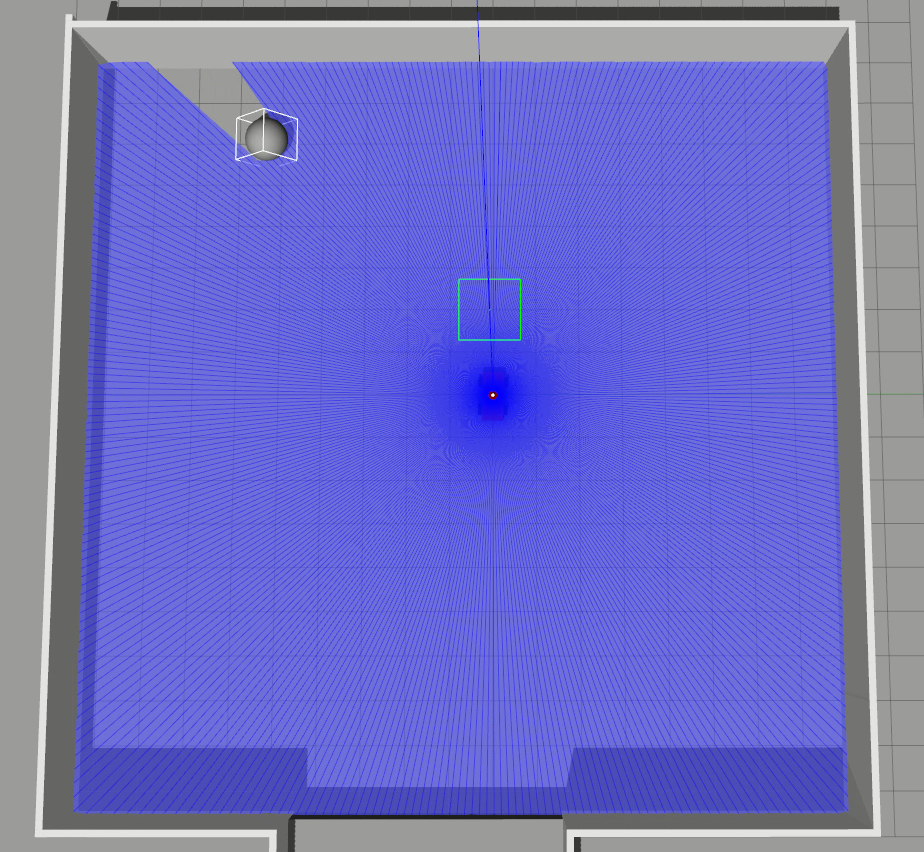
\includegraphics[height=70mm]{figures/raw/mapping_demo/gazebo_ball_moving.png}
        \label{mapping_demo_gazebo_ball_moving}
    }
    \subfloat[rviz visualization]
    {
    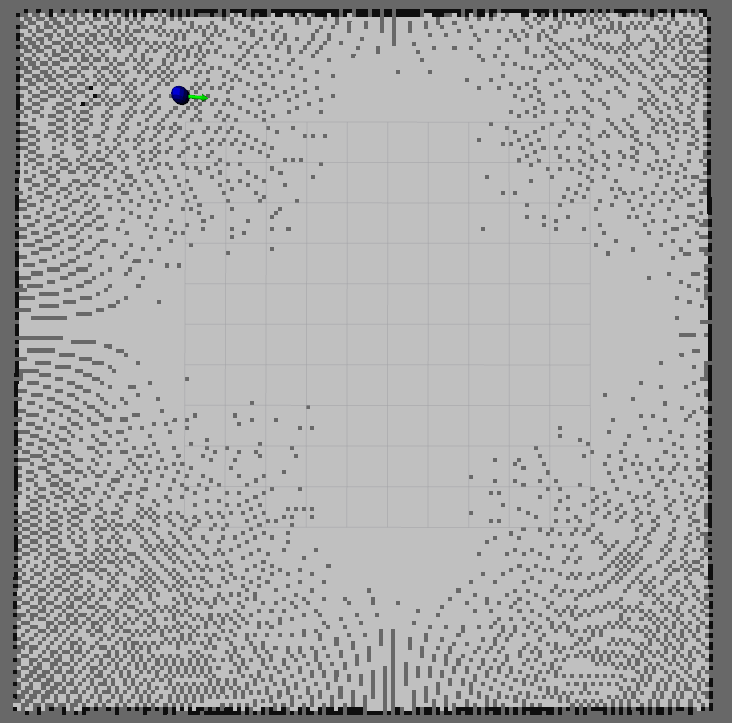
\includegraphics[height=70mm]{figures/raw/mapping_demo/rviz_ball_moving.png}
        \label{mapping_demo_rviz_ball_moving}
    }
    \caption{The ball is moving}
    \label{mapping_demo_ball_moving}
\end{figure}

When the car starts moving, the map immediately starts to clear out. If we compare \ref{mapping_demo_ball_moving} and \ref{mapping_demo_car_moving}, it is clear that the latter contains less unknown grid points.

\begin{figure}[!ht]
    \centering
    \subfloat[Gazebo simulation]
    {
        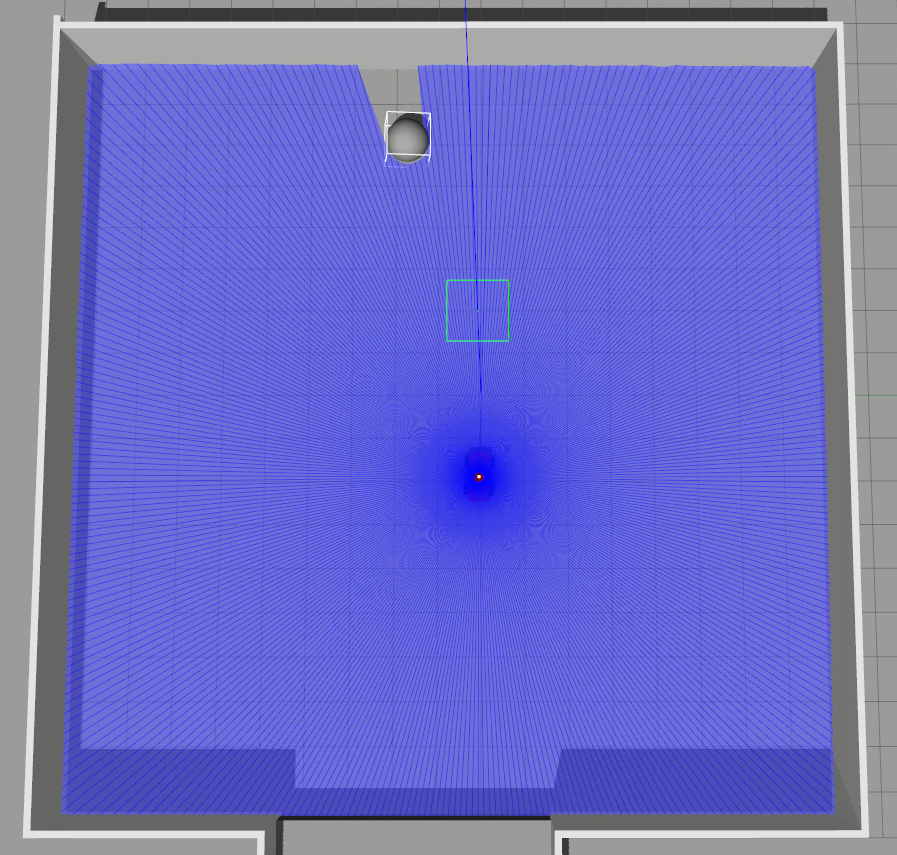
\includegraphics[height=70mm]{figures/raw/mapping_demo/gazebo_car_moving.png}
        \label{mapping_demo_gazebo_car_moving}
    }
    \subfloat[rviz visualization]
    {
    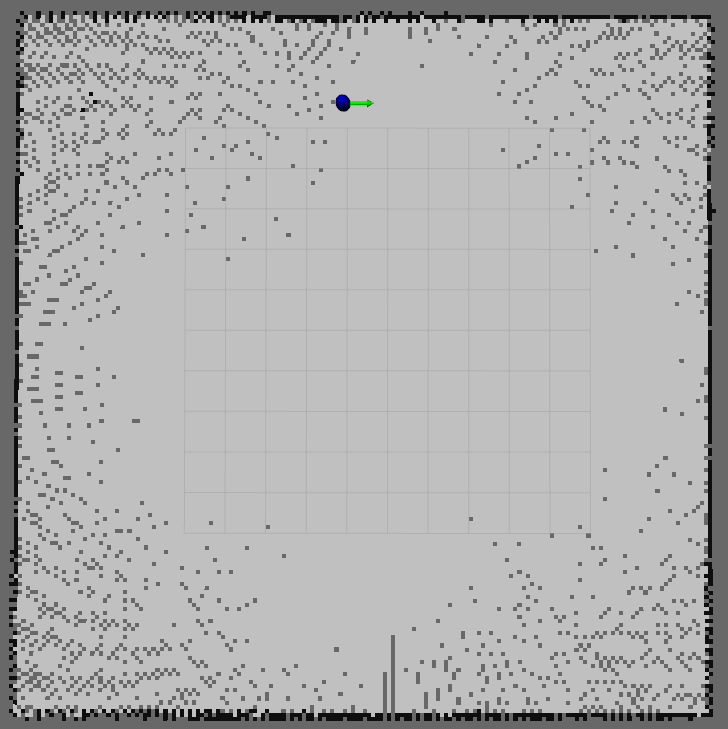
\includegraphics[height=70mm]{figures/raw/mapping_demo/rviz_car_moving.png}
        \label{mapping_demo_rviz_car_moving}
    }
    \caption{The car is moving}
    \label{mapping_demo_car_moving}
\end{figure}

Due to the map implementation being very simple, and updating each map point without handling its history, the mapping node can only be used with certain limitations regarding obstacle speed and the car's angular velocity. But the main task for the mapping algorithm was not to create a static map with the best possible quality, but to separate the static points from the dynamic objects.

\section{Motion planning results}
The task of the motion planning node was to calculate and publish actuations based on the static and dynamic maps provided by the mapping node, that lead the car towards the destination, following the required trajectory, without any collisions. The algorithm first filters the static and dynamic input maps to decrease the number of environment points. Then it calculates trajectories for the dynamic obstacles. Independently from the maps, it sets the target actuation according to the target trajectory or an external control command, and also updates the dynamic window, based on the current actuation. When all these steps are finished, it calculates the collision times for all the actuations in the dynamic window and all objects in the car's environment, and builds the velocity obstacle map. Using this map and the target actuation, fitness factors are calculated for all available actuations. Summarizing and evaluating these factors, the best possible actuation is determined. This actuation is then published to the actuator nodes.

\section{Interesting findings and morals}
During the implementation of the mapping and planning algorithms I had to face a few problems that I thought was worth mentioning, either because they were surprisingly hard to overcome or just because they were unexpected or interesting.

\subsection{Symmetrical map}
The first one is rather a tip than a finding - a tip for myself in the future and anyone who is planning on writing a mapping program. \textit{Don't use a symmetrical map, with the car starting in its center!} Build an asymmetrical map or place the car somewhere but the center. It took me at least 3 hours of debugging to find where one of the absolute point angle calculations was wrong, that cause the  map to rotate by 180 degrees. But for quite a long time, this bug didn't event come to my attention, because the map was symmetrical, and therefore was insensitive to a 180 degree rotation.

\subsection{The closing ball}
The second finding is an unexpected mapping problem that I didn't event notice until it ruined the local trajectory planning. It happened when a round object\footnote{In the simulator I used balls as obstacles, because applying a still force to them made them move with a linear speed.} is moving in a straight line, and passes near the car. Because of its round shape, only a half of the object is seen by the LIDAR at every time point. But the half that is visible is changing as the object is passing the car (kind of like the Sun making different parts of the Moon visible, as it's rotating relative to the Earth). But the speed vector calculation is based on the movement of the objects' mass center, which is calculated by the visible points. Therefore, as the visible points select a different half of the object, the mass center changes, and alters the object's speed vector. In figure \ref{closing_ball} this effect can be viewed. The ball is moving in a straight line, its speed vectors in every step are marked with the black arrows. The visible points (marked with red dots) are shifting to the side of the ball as it passes the car. As a result, the calculated speed vectors (green arrows) tend to 'bend' towards the car when the obstacles is getting closer.

The effect of the speed vectors changing does not seem relevant, but during motion planning, the ball is seen as an object that is moving forward, but suddenly, it starts to approach the car by turning more and more towards it, making all actuations to be marked unsafe.

The problems has not been solved entirely, but its effect has been reduced by changing the mass center calculation method in the mapping node.

\begin{figure}[!ht]
    \centering
    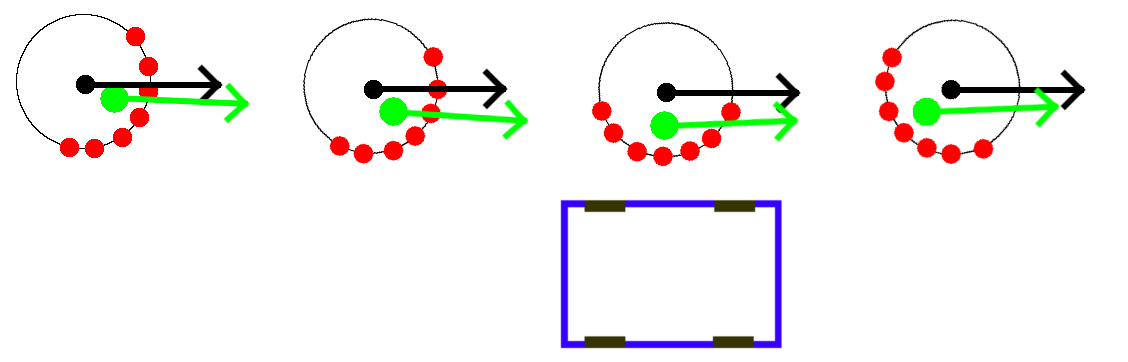
\includegraphics[height=40mm]{figures/raw/closing_ball.png}
    \caption{The closing ball}
    \label{closing_ball}
\end{figure} 